\subsubsection{UC7 - Acquisto beni}
\begin{figure}[h]
	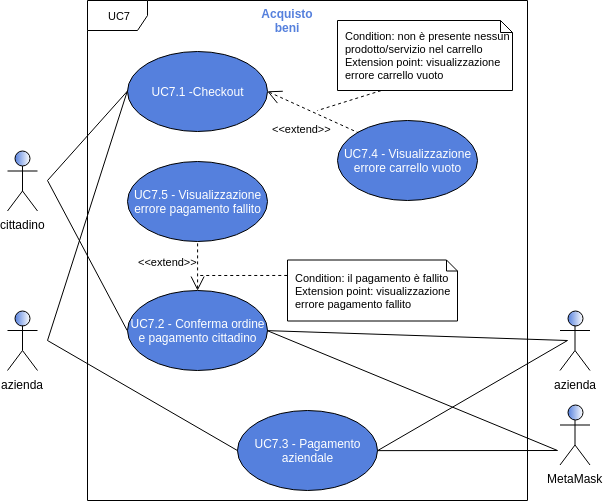
\includegraphics[width=10cm]{res/images/UC7-Generale.png}
	\centering
	\caption{UC7 - Acquisto beni}
\end{figure}
\begin{itemize}
	\item \textbf{Attori Primari}: cittadino e azienda-cliente;
	\item \textbf{Attori Secondari}: azienda-venditrice, MetaMask\glo;
	\item \textbf{Descrizione}: i cittadini e le aziende possono acquistare i prodotti/servizi che avevano precedentemente aggiunto nel carrello;
	\item \textbf{Scenario principale}: 
	\begin{enumerate}[label=\alph*.]
		\item l'utente inserisce dei prodotti nel carrello [UC6.1];
		\item l'utente procede con il checkout dei prodotti precedentemente inseriti [UC7.1];
		\item l'utente sceglie l'indirizzo di spedizione [UC7.3];
		\item l'utente effettua la conferma ed il pagamento dell'ordine [UC7.4];
	\end{enumerate}
	
	\item \textbf{Precondizione}: il sistema ha reso disponibile all'utente l'utilizzo del carrello per poter effettuare degli acquisti. L'utente ha inserito degli oggetti nel carrello ed ha espresso la volontà di acquistare tali prodotti;
	\item \textbf{Postcondizione}: è stato effettuato l'acquisto dei beni presenti nel carrello. Viene applicato il meccanismo di escrow\glo. Il cliente riceve la conferma d'acquisto\glo. Entro la data ultima di approvazione esso potrà approvare o rifiutare l'ordine. I soldi del pagamento sono temporaneamente trattenuti nella piattaforma.
\end{itemize} 
\subsubsection{UC7.1 - Checkout}
\begin{itemize}
	\item \textbf{Attori Primari}: cittadino, azienda;
	\item \textbf{Descrizione}: l'utente effettua il checkout per poter poi acquistare i prodotti inseriti nel carrello;
	\item \textbf{Scenario principale}: l'utente preme il pulsante per effettuare il checkout;
	\item \textbf{Estensioni}: 
	\begin{itemize}
		\item \textbf{UC7.2}: l'utente preme il pulsante di checkout senza aver ancora inserito almeno un prodotto/servizio nel carrello;
	\end{itemize}
	\item \textbf{Precondizione}: il sistema ha reso disponibile il carrello all'utente, identificandolo quindi come cittadino o azienda. L'utente ha espresso la volontà di procedere con il checkout premendo l'apposito pulsante;
	\item \textbf{Postcondizione}: l'utente accede alla pagina dove poter confermare l'acquisto e procedere con il pagamento.
\end{itemize}

\subsubsection{UC7.2 - Visualizzazione errore carrello vuoto}
\begin{itemize}
	\item \textbf{Attori Primari}: azienda;
	\item \textbf{Descrizione}:
	l'utente visualizza un messaggio di errore relativo al fatto che non è presente alcun prodotto nel proprio carrello e che quindi non è possibile procedere con la procedura di checkout;
	\item \textbf{Scenario}: l'utente tenta di procedere con il checkout senza aver inserito alcun prodotto/servizio nel carrello;
	\item \textbf{Precondizione}: il sistema ha reso disponibile all'utente il carrello ed il pulsante di checkout. L'utente ha premuto sul pulsante di checkout ed il carrello risulta vuoto; 
	\item \textbf{Postcondizione}:
	l'utente è consapevole che, per procedere con il checkout, il carrello deve contenere almeno un prodotto/servizio. 
\end{itemize}

\subsubsection{UC7.3 - Scelta indirizzo spedizione}
\begin{itemize}
	\item \textbf{Attori Primari}: azienda, cittadino;
	\item \textbf{Descrizione}:
	l'utente dopo aver effettuato il checkout deve selezionare l'indirizzo di spedizione. Gli vengono presentate due possibilità:
	\begin{itemize}
		\item utilizzare l'indirizzo inserito durante la registrazione;
		\item inserire un nuovo indirizzo da utilizzare per questa spedizione, inserendo le informazioni relative ad un indirizzo [UC2.2.2];
	\end{itemize}
	\item \textbf{Scenario principale}: l'utente dopo aver richiesto il checkout, per continuare nel procedimento di acquisto, deve selezionare un indirizzo di spedizione;
	\item \textbf{Precondizione}: l'utente ha eseguito il checkout;
	\item \textbf{Postcondizione}:
	l'utente ha inserito l'indirizzo di spedizione e può continuare concludendo il procedimento di acquisto. Tale indirizzo verrà utilizzato per la creazione della relativa fattura.
\end{itemize}



\subsubsection{UC7.4 - Conferma ordine e pagamento}
\begin{itemize}
	\item \textbf{Attori Primari}: azienda-cliente;
	\item \textbf{Attori Secondari}: azienda-venditrice, MetaMask\glo;
	\item \textbf{Descrizione}: l'utente, dopo aver selezionato l'indirizzo di spedizione, procede con la conferma ed il pagamento dell'ordine;
	\item \textbf{Scenario principale}: l'utente conferma l'ordine premendo l'apposito pulsante. Segue dunque la procedura di pagamento attraverso l'utilizzo del plugin MetaMask\glo;
	\item \textbf{Estensioni}: 
	\begin{itemize}
		\item \textbf{UC7.4}: l'esito del pagamento da parte del plugin MetaMask\glosp risulta negativo, l'utente riceve un messaggio di errore che lo invita a controllare la causa dello stesso direttamente dal plugin; 
	\end{itemize}
	\item \textbf{Precondizione}: l'utente ha effettuato il checkout e la selezione dell'indirizzo di spedizione;
	\item \textbf{Postcondizione}: il pagamento è avvenuto con successo. L'importo della transazione momentaneamente è trattenuto dal sistema a causa del meccanismo di escrow\glo. Il cliente riceve nella pagina dedicata la conferma d'acquisto\glo. L'azienda-venditrice riceve nella pagina dedicata l'ordine non ancora confermato relativo al suddetto.
\end{itemize}


\subsubsection{UC7.5 - Visualizzazione errore pagamento fallito}
\begin{itemize}
	\item \textbf{Attori Primari}: azienda;
	\item \textbf{Attori Secondari}: MetaMask\glo;
	\item \textbf{Descrizione}:
	l'utente visualizza un messaggio di errore relativo al fatto che il tentativo di pagamento non è andato a buon fine, e che quindi l'ordine è stato annullato. L'utente viene invitato ad informarsi sulla causa del fallimento dell'operazione all'interno del plugin.
	\item \textbf{Scenario principale}: l'utente tenta pagare attraverso il plugin MetaMask\glosp la somma dovuta al venditore per l'acquisto corrente;
	\item \textbf{Precondizione}: il sistema permette all'utente di procedere con il pagamento, ovvero l'ordine è stato confermato da parte dell'utente;
	\item \textbf{Postcondizione}:
	l'utente è consapevole che l'acquisto non è andato a buon fine, e che per ottenere informazioni più precise dovrà riferirsi al messaggio di errore riportato nel plugin. 
\end{itemize} 






